\chapter{はじめに}
被災地での救助活動を行う際に,訓練されたレスキュー犬(災害救助犬)が人間の補助として探査を行う場合がある~(図~\ref{resque}).
災害救助犬を育成し、現場に派遣する団体は日本国内に複数存在し,必要に応じて現場に派遣される.
レスキュー犬は,犬としての特性を生かして人間と協力して被災地の探索を行う.
レスキュー犬にはがれきの隙間などの狭い空間,倒壊した建築物など人間には踏破困難な環境でも探査可能であったり,またその発達した嗅覚を頼りにした探査が可能である.このように,人間では探査が困難あるいは不可能な環境においても人間の能力をレスキュー犬が補うことで効果的な救助活動が期待される.
しかし,彼らレスキュー犬は人間に向けた言語を持たない.そのため,人間はレスキュー犬の行動をよく観察し,彼らが収集した情報を彼らの様子から推察,理解しなくてはならない.
現状では,レスキュー犬を直接指揮するハンドラーと呼ばれる人間がレスキュー犬の行動を手動でマーキングして犬の周辺環境の情報収集と理解に努めている.
収集された情報は消防などのハンドラーらを統括する指揮命令者に口頭伝達され,現場の把握に活かされる.
このレスキュー犬と人間との共同探索の問題点として,トリアージ(緊急度に従った手当の優先順位付け)のための災害現場周辺環境情報や,要救助者情報の不足があげられる.
また,ハンドラーによる記録はどうしても主観的になるので客観性に欠け,さらにそれが口頭伝達されることで正確性がより欠落する.
レスキュー犬によって収集された情報を個人の主観に基づくことなく分類し,整理された情報を共有できれば災害救助活動の効率化がより期待される.

本研究では,レスキュー犬にセンサを装着して得られた一人称動画を用いてレスキュー犬の行動を分類すること目的とする.
本研究では最初に深層学習を用いた画像認識手法を,一人称映像から抽出した静止画像に適用して動作分類を行う予備実験を行った.
この予備実験で犬一人称視点映像からの動作分類タスクに対してCNNを用いた推定が有効が有効であることを確認した.
予備実験をもととし,静止画像に加えて一人称画像から抽出した動き情報と音声情報を利用したマルチモーダルなレスキュー犬行動推定を行った.
本研究により,レスキュー犬が今何をしているのかハンドラーが目視できない場合でも機械的に判断することが可能となり,トリアージに必要な情報が整理され,災害救助活動の効率化が期待される.
\begin{figure}[htbp]
 \begin{center}
  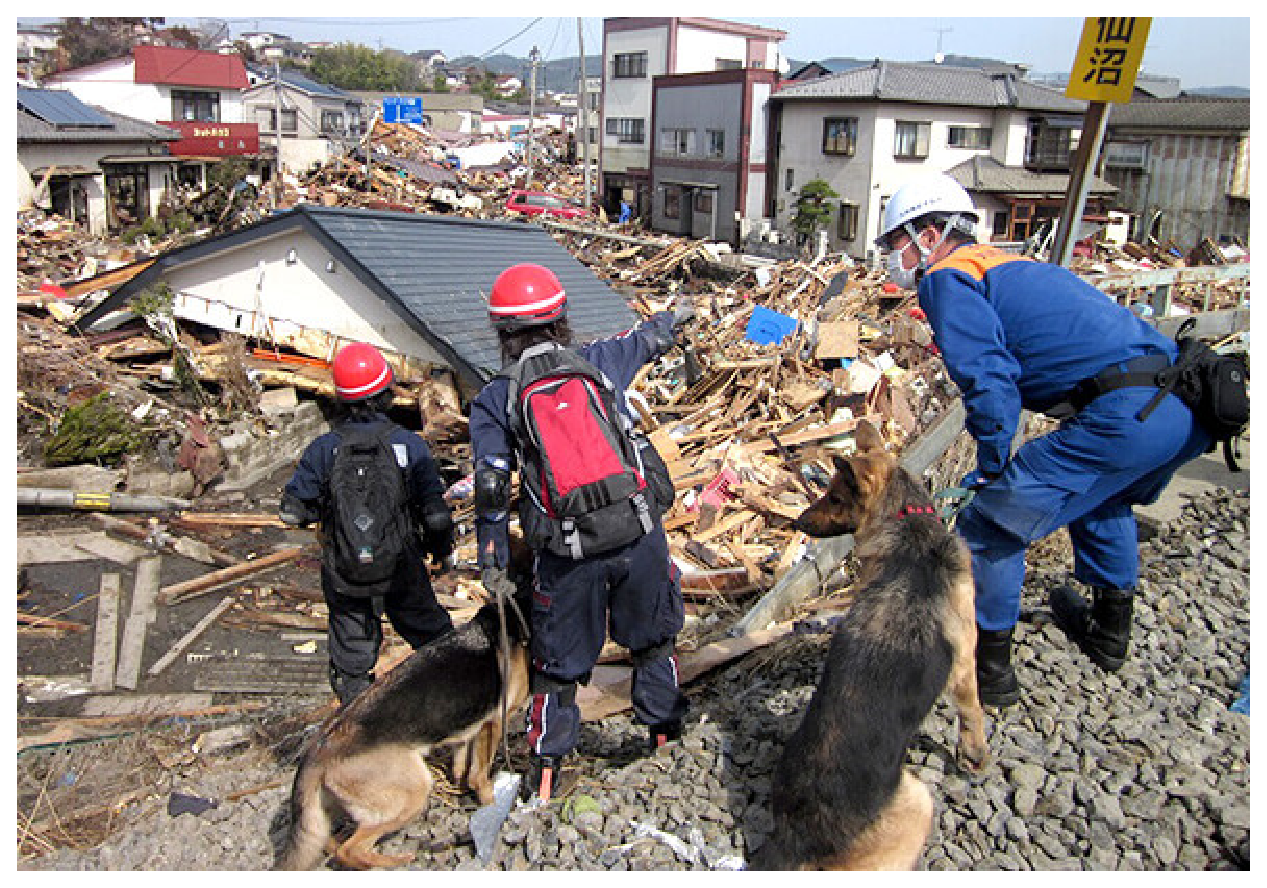
\includegraphics[width=12cm]{./Figures/resque.eps}
  \caption{被災地におけるレスキュー犬らの救助活動~\cite{buycott}より引用}
  \label{resque}
 \end{center}
\end{figure}
